\chapter{Implementazione}

In questo capitolo verrà presentato nel dettaglio l'implementazione del database e del web service.

\section{Struttura dell'applicazione}

\begin{figure}[H]
	\centering
	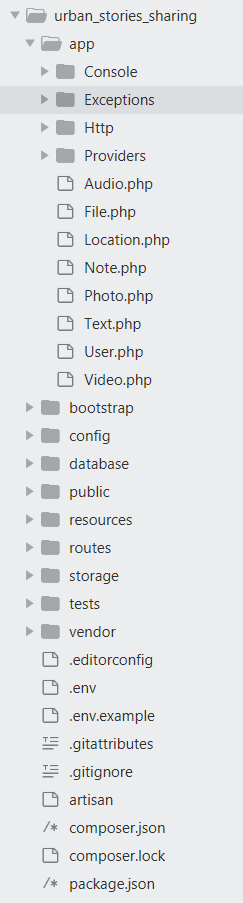
\includegraphics[width=0.3\linewidth, height=0.4\textheight]{Struttura_applicazione}
	\caption{Struttura dell'applicazione}
	\label{fig:Strutturaapplicazione}
\end{figure}


La struttura dell'applicazione lato back-end, come si può vedere in Figura 3.1, mantiene la struttura base di un'applicazione Laravel, strutturata in cartelle, ognuna delle quali contiene dei files con uno specifico compito.

\subsection{App directory}
\begin{figure}[H]
	\centering
	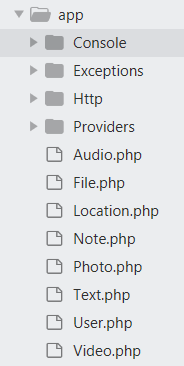
\includegraphics[width=0.15\linewidth, height=0.2\textheight]{AppDirectory}
	\caption{App directory}
	\label{fig:appdirectory}
\end{figure}
La cartella \textit{\textbf{app}} contiene il codice principale dell'applicazione. Per impostazione predefinita del framework, questa directory è assegnata sotto il namespace di \textbf{App} e viene caricata automaticamente da Composer.
Questa directory contiene tutti i modelli definiti per lo sviluppo del progetto oltre a varie sotto directory aggiuntive come Console e Http, che si possono considerare come un vero e proprio strato che fornisce un'API nel nucleo dell'applicazione.
La directory Console contiene tutti i comandi Artisan personalizzati, mentre la directory Http contiene controller e middleware, ovvero tutta logica per gestire le richieste.

\subsection{Database directory}
\begin{figure}[H]
	\centering
	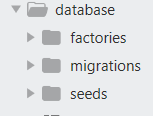
\includegraphics[width=0.2\linewidth, height=0.1\textheight]{DatabaseDirectory}
	\caption{Database directory}
	\label{fig:databasedirectory}
\end{figure}

La direcory \textit{\textbf{Database}} contiene le migrazioni della base di dati e i file di \textit{\textbf{seeds}}, utili a popolare il modello.

\subsection{Storage directory}
La directory di archiviazione contiene l'archivio \textit{\textbf{/app/directory}} pubblico, il quale, viene utilizzato per archiviare file generati dall'utente, ovvero le note contenenti i file multimediali, che devono essere accessibili al pubblico. 

\section{Implementazione database}
Inizialmente, per quanto concerne la creazione del modello relazione, si era pensato di predisporre una entità autonoma per ogni tipo di file multimediale da caricare sul database, ma questo tipo di soluzione risultava ridondante poichè diverse entità presentavano gli stessi attributi, per questo motivo si è deciso di cambiare approccio e utilizzare un'entità genitore \textbf{files}, contenente le informazioni comuni, in relazione alle entità specializzanti per ogni tipo di file: \textbf{photos}, \textbf{audios} e \textbf{videos}. 
\begin{lstlisting}[caption = Esempio schema tabella files]
public function up()
{
	Schema::create('files', function (Blueprint $table) 
	{
		$table->increments('id');
		$table->float('size');
		$table->text('format');
		$table->mediumText('path')->nullable();
		$table->integer('note_id')->unsigned();
		$table->integer('photo_id')->unsigned()
			->unique()->nullable();
		$table->integer('audio_id')->unsigned()
			->unique()->nullable();
		$table->integer('video_id')->unsigned()
			->unique()->nullable();
		$table->foreign('note_id')->references('id')
			->on('notes');
		$table->foreign('photo_id')->references('id')
			->on('photos');
		$table->foreign('audio_id')->references('id')
			->on('audios');
		$table->foreign('video_id')->references('id')
			->on('videos');
		$table->timestamps();
	});
}
\end{lstlisting}
\begin{lstlisting}[caption=Esempio schema tabella videos]
public function up()
{
	Schema::create('videos', function (Blueprint $table) 
	{
		$table->increments('id');
		$table->integer('duration');
		$table->integer('width');
		$table->integer('height');
		$table->integer('bit_rate');
		$table->integer('frame_rate');
		$table->timestamps();
	});
}
\end{lstlisting}
Con lo sviluppo del progetto si è deciso di aggiungere, al modello, una nuova entità \textit{\textbf{notes}} messa in relazione con l'entità \textit{\textbf{files}}, \textit{\textbf{texts}} e \textit{\textbf{locations}}, rappresentante la geolocalizzazione delle note, che inizialmente era in relazione con l'entità \textit{\textbf{files}}.

\subsection{Codifica dei dati}
La codifica dei dati è un punto critico del progetto, poichè una scelta implementativa non ottimale potrebbe appensantire molto la base di dati.
Le due alternative possibili erano l'upload tramite \textit{\textbf{multipart form-data}} oppure tramite la \textbf{codifica in base64}.

Dopo un'analisi delle ipotetiche dimensioni dei file salvate nel repository, si è scelto di riceve i dati codificati in \textbf{Base64}, poiché si presuppone che le note testuali, le immagini, i file audio e i file video caricati sul server siano di piccole dimensioni.
Inoltre è stato scelto di non salvare la codifica dei dati nel database, per evitare, una volta raggiunti volumi importanti di dati, di appesantire la base di dati.
Per permettere, nonostante ciò, al client, di ricevere il file richiesto con richieste HTTP di tipo \textit{\textbf{GET}}, il server si preoccupa di codificare i dati prima di essere inviati al client.

\pagebreak
\section{Implementazione web service}

Questa sezione tratta dell'implementazione del web service sviluppato per lo scambio di informazioni con la parte client, in particolare si mostrerà come vengono salvati e recuperati i file.

\subsection{Routes}

\begin{lstlisting}[caption={Definizione routes}]
	Route::get('/notes', 'NoteController@index');
	Route::get('/notes/{id}', 'NoteController@show');
	Route::get('/texts/{id}', 'TextController@show');
	Route::post('/texts', 'TextController@store');
	Route::get('/photos/{id}', 'PhotoController@show');
	Route::post('/photos', 'PhotoController@store');
	Route::get('/audios/{id}', 'AudioController@show');
	Route::post('/audios', 'AudioController@store');
	Route::get('/files/{id}', 'FileController@show');
	Route::get('/videos/{id}', 'VideoController@show');
	Route::post('/videos', 'VideoController@store');
\end{lstlisting}

Le routes definite vengono caricate dal \textbf{RouteServiceProvider} a cui è assegnato il gruppo middleware 'api' e si occupano di instradare le richieste sui vari endpoint verso il controller dedicato.

\subsection{Controllers}

Definite le routes, sono stati realizzati i vari controller. Per ogni tipologia di file caricabile è stato definito un controller che gestisce le varie operazioni di richiesta e salvataggio dati.
Per ogni controller, quindi, sono stati definiti gli opportuni metodi che gestiscono le varie richieste HTTP;
I nomi dei metodi definiti all'interno dei controller sono stati standardizzati in modo da permettere una più semplice comprensione.

\pagebreak
\subsubsection{Metodo Index}
Il metodo \textit{\textbf{index}}, all'interno di un controller, risponde ad una richiesta di tipo \textit{\textbf{GET}} e si occupa di recuperare i file richiesti dal database. Il metodo può ritornare una collezione di oggetti specifici, identificati dai parametri passati tramite query string oppure una collezione di tutte le note registrate nel database.

\subsubsection{Metodo Store}
l metodo \textit{\textbf{store}} si occupa della gestione delle richieste HTTP di tipo \textit{\textbf{POST}}. 
Ovvero gestisce tutte le operazioni di salvataggio di ogni tipo di files.

\subsubsection{Metodo Show}
\begin{lstlisting}[caption={Funzione Show del controller NoteController}]
public function show($id) 
{
	if(Note::find($id)){
		return Note::find($id);
	}else {
		return Response('Note not found', 404);
	}
}
\end{lstlisting}

Il un metodo \textit{\textbf{show}} gestisce richieste HTTP di tipo \textit{\textbf{GET}} e ritorna un oggetto singolo che corrisponde ad un file, identificato dal parametro \textit{\textbf{id}} passato con la richiesta; il tipo dell'oggetto ritornato dipende dall'endpoint su cui si effettua la richiesta.

\subsubsection{Query string}
Quando viene effettuata una richiesta HTTP di tipo \textit{\textbf{GET}} può essere necessario passare dei parametri in \textit{\textbf{query string}} per specificare una certa tipologia di files da reperire.
Per permettere questo tipo di operazioni è stata implementata la gestione, appunto, delle query string.
La richiesta principale è quella di reperire delle note entro una certa distanza da una posizione data; La logica alla base di questa operazione è quella di ottenere tutti i parametri passati in query string, ovvero le coordinate geografiche dell'utente e la distanza massima entro la quale si vogliono recuperare i dati; dopodichè, vengono ciclate tutte le note all'interno del repository e, sfruttando il teorema di Pitagora, vengono selezionate solo le note richieste.

\begin{lstlisting}[caption={Gestione query string}]
foreach ($notes as $key => $value) {

	if($value->location != null) {
		$lat2 = $value->location->latitude;
		$long2 = $value->location->longitude;
		$distance = sqrt(
				pow($lat2-$lat1, 2) +
			 	pow($long2-$long1, 2)
			 	);

		if($distance > $max_distance) {
			$notes->forget($key);
		}    
	} else {
		$notes->forget($key);
	}
}
\end{lstlisting}

